% Section 3: Results

\section{Results}

This section compares xRFM with XGBoost, LightGBM, and MLP in terms of predictive performance, scalability, and interpretability. All models are evaluated under the same preprocessing, train-validation-test split, and metrics defined in Section~2.

\subsection{Predictive Performance}

Table~\ref{tab:main-results} reports the final held-out test performance across all five datasets. RMSE is used for regression tasks, while accuracy and AUC-ROC are used for binary classification tasks. Bold values indicate the best result for each metric.

\begin{table}[htbp]
  \centering
  \caption{Test-set performance of all models. \textbf{Bold} indicates best result per dataset and metric. RMSE is lower-better; Accuracy and AUC are higher-better.}
  \label{tab:main-results}
  \begin{tabular}{llcccc}
    \toprule
    \multirow{2}{*}{Dataset} & \multirow{2}{*}{Metric}
      & \multicolumn{4}{c}{Model} \\
    \cmidrule(lr){3-6}
      & & xRFM & XGBoost & LightGBM & MLP \\
    \midrule
    Diamonds
      & RMSE $\downarrow$
        & 1496.72 & 544.68 & \textbf{535.99} & 734.69 \\[2pt]
    Superconductivity
      & RMSE $\downarrow$
        & 9.454 & 9.302 & \textbf{9.209} & 11.066 \\[4pt]
    \multirow{2}{*}{Online Shoppers}
      & Accuracy $\uparrow$ & 0.8897 & 0.9031 & \textbf{0.9039} & 0.8946 \\
      & AUC $\uparrow$      & 0.9018 & \textbf{0.9306} & 0.9306 & 0.9040 \\[2pt]
    \multirow{2}{*}{Stroke}
      & Accuracy $\uparrow$ & 0.9413 & 0.9491 & 0.9501 & \textbf{0.9511} \\
      & AUC $\uparrow$      & 0.7605 & \textbf{0.8388} & 0.8231 & 0.2690 \\[2pt]
    \multirow{2}{*}{HR Attrition}
      & Accuracy $\uparrow$ & \textbf{0.8673} & 0.8571 & 0.8469 & 0.8639 \\
      & AUC $\uparrow$      & 0.7631 & 0.7552 & \textbf{0.7886} & 0.7512 \\
    \bottomrule
  \end{tabular}
\end{table}

\paragraph{Regression tasks.}
LightGBM achieves the lowest RMSE on both regression datasets. xRFM is close on Superconductivity (9.454 vs.\ 9.209) but far behind on Diamonds (1496.72 vs.\ 535.99), indicating that AGOP-based feature learning does not automatically generalise to large mixed-type regression.

\paragraph{Classification tasks.}
XGBoost and LightGBM achieve the best AUC-ROC on Online Shoppers and Stroke. xRFM's strongest result is HR Attrition, where it achieves the highest accuracy (0.8673), suggesting a modest advantage in small-sample settings. MLP has notably low AUC on Stroke (0.269), reflecting sensitivity to class imbalance.

Table~\ref{tab:timing} reports training time and per-sample inference time for all models and datasets.

\begin{table}[htbp]
  \centering
  \caption{Training time (s) and inference time per sample ($\mu$s) for all models. Each cell shows Train\,/\,Infer.}
  \label{tab:timing}
  \small
  \resizebox{\textwidth}{!}{
  \begin{tabular}{lrrrr}
    \toprule
    Dataset & xRFM & XGBoost & LightGBM & MLP \\
    \midrule
    Diamonds           & 246.5\,s / 69.8\,$\mu$s & 1.4\,s / 1.9\,$\mu$s & 0.8\,s / 1.9\,$\mu$s & 26.8\,s / 0.9\,$\mu$s \\
    Superconductivity  & 1.6\,s / 1.0\,$\mu$s   & 3.4\,s / 2.1\,$\mu$s & 1.9\,s / 7.6\,$\mu$s & 34.3\,s / 0.8\,$\mu$s \\
    Online Shoppers    & 0.7\,s / 0.8\,$\mu$s   & 0.2\,s / 1.4\,$\mu$s & 0.3\,s / 1.6\,$\mu$s & 2.1\,s / 0.8\,$\mu$s  \\
    Stroke             & 0.3\,s / 1.1\,$\mu$s   & 0.1\,s / 1.1\,$\mu$s & 0.1\,s / 2.0\,$\mu$s & 0.4\,s / 1.0\,$\mu$s  \\
    HR Attrition       & 0.1\,s / 3.2\,$\mu$s   & 0.1\,s / 3.0\,$\mu$s & 0.1\,s / 7.5\,$\mu$s & 0.4\,s / 2.2\,$\mu$s  \\
    \bottomrule
  \end{tabular}
  }
\end{table}

\subsection{Scalability Analysis}

To evaluate scalability, we run subsampling experiments on Diamonds and Superconductivity. Table~\ref{tab:scaling} reports RMSE and training time at different training sizes. Figure~\ref{fig:scaling} visualises the scaling curves for both datasets.

\begin{table}[htbp]
  \centering
  \caption{Scalability experiment: test RMSE and training time (seconds) as a function of training set size. Dash (--) indicates configurations not run.}
  \label{tab:scaling}
  \resizebox{\textwidth}{!}{
  \begin{tabular}{llrrrrrrrr}
    \toprule
    \multirow{2}{*}{Dataset} & \multirow{2}{*}{$n_\text{train}$}
      & \multicolumn{2}{c}{xRFM} & \multicolumn{2}{c}{XGBoost} & \multicolumn{2}{c}{LightGBM} & \multicolumn{2}{c}{MLP} \\
    \cmidrule(lr){3-4}\cmidrule(lr){5-6}\cmidrule(lr){7-8}\cmidrule(lr){9-10}
      & & RMSE & Time (s) & RMSE & Time (s) & RMSE & Time (s) & RMSE & Time (s) \\
    \midrule
    \multirow{4}{*}{Diamonds}
      & 1{,}000  & 1657.0 &   0.77 & 846.7 & 0.80 & 1003.4 & 0.13 & 1081.0 &  2.27 \\
      & 5{,}000  & 1655.9 &  11.03 & 628.9 & 0.39 &  622.7 & 0.11 &  901.1 & 10.12 \\
      & 10{,}000 & 1577.6 &  39.31 & 587.8 & 0.49 &  592.3 & 0.15 &  888.9 & 10.33 \\
      & 30{,}000 & 1487.5 & 226.44 & 542.7 & 0.59 &  535.3 & 0.29 &  743.5 & 22.23 \\[4pt]
    \multirow{4}{*}{Supercond.}
      & 1{,}000  & 14.07 & 0.08 & 13.76 & 0.39 & 13.91 & 0.15 & 15.39 &  2.52 \\
      & 5{,}000  & 11.30 & 0.47 & 10.81 & 1.00 & 10.71 & 0.46 & 13.05 &  8.58 \\
      & 10{,}000 &  9.81 & 1.07 &  9.51 & 1.73 &  9.50 & 1.10 & 11.22 & 28.35 \\
      & 12{,}757 &  9.46 & 1.56 &  9.28 & 1.64 &  9.21 & 1.04 & -- & -- \\
    \bottomrule
  \end{tabular}
  }
\end{table}

\begin{figure}[htbp]
  \centering
  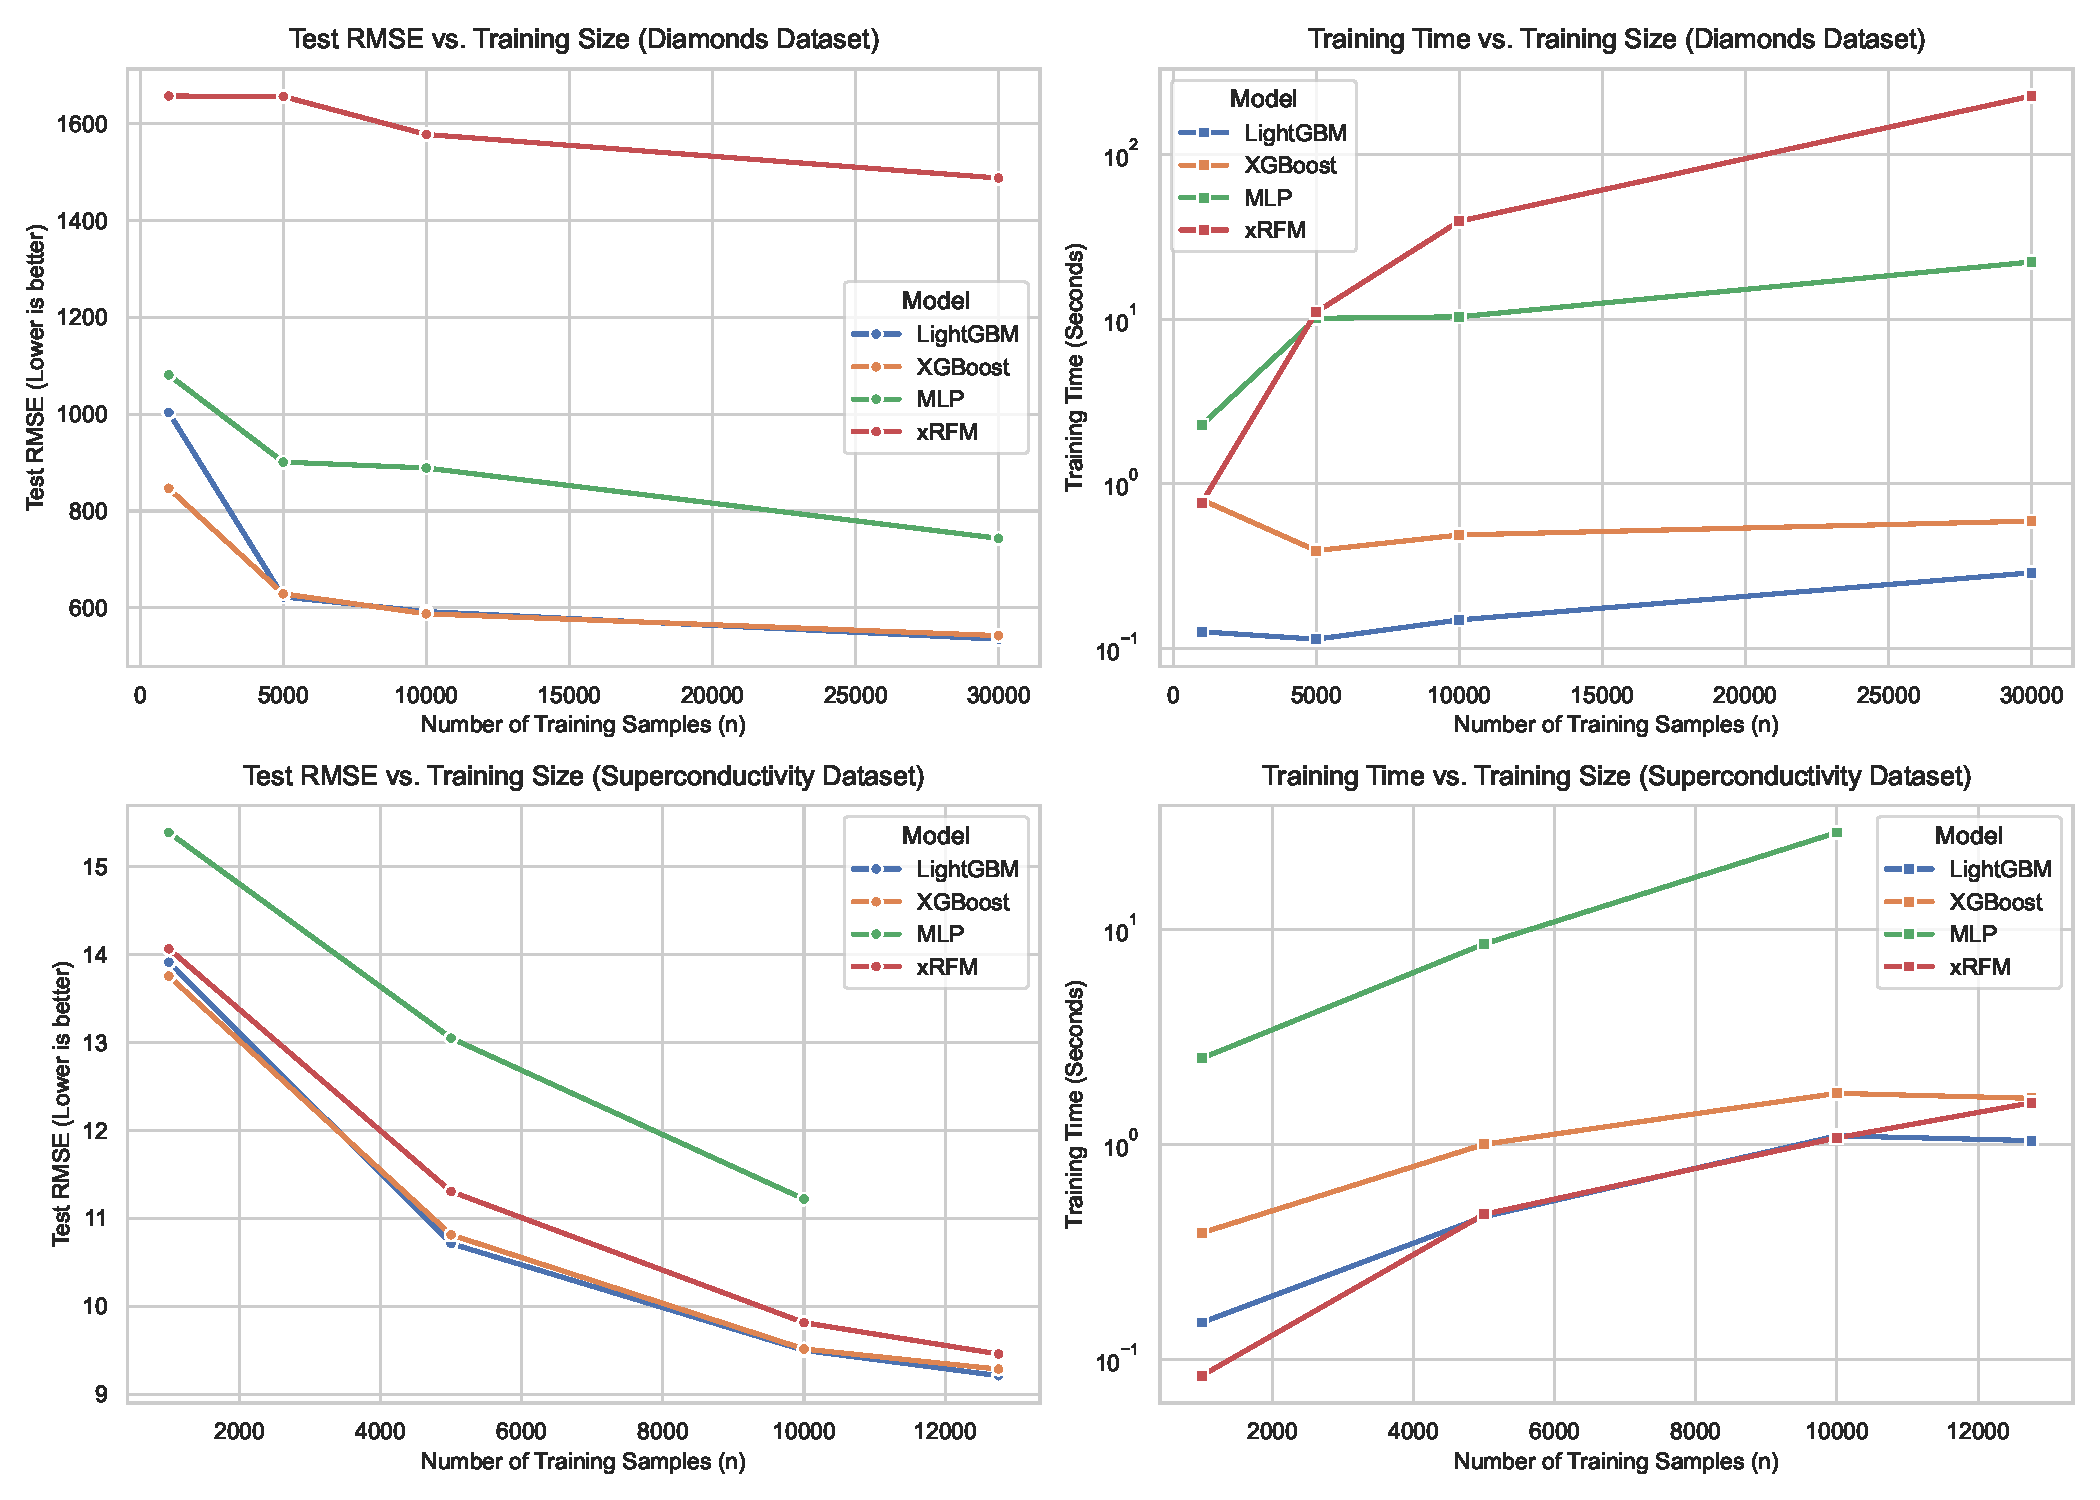
\includegraphics[width=\textwidth]{figures/scaling_analysis_2x2.pdf}
  \caption{Scalability analysis across Diamonds and Superconductivity datasets. The left column shows test RMSE, while the right column shows training time (in log-scale) as a function of training set size. This illustrates xRFM's steeper time complexity compared to the tree-based models.}
  \label{fig:scaling}
\end{figure}

On Diamonds, xRFM's training time grows from 0.77s to 226.44s as $n$ increases from 1{,}000 to 30{,}000, while its RMSE only improves from 1657.0 to 1487.5; LightGBM reaches 535.3 in under one second. On Superconductivity, xRFM scales more favourably, improving from 14.07 to 9.46 RMSE over the same range. As shown in Figure~\ref{fig:tradeoff}, the Pareto front analysis confirms that while xRFM approaches the performance of LightGBM on numerical datasets, it requires exponentially more training time.

\begin{figure}[htbp]
  \centering
  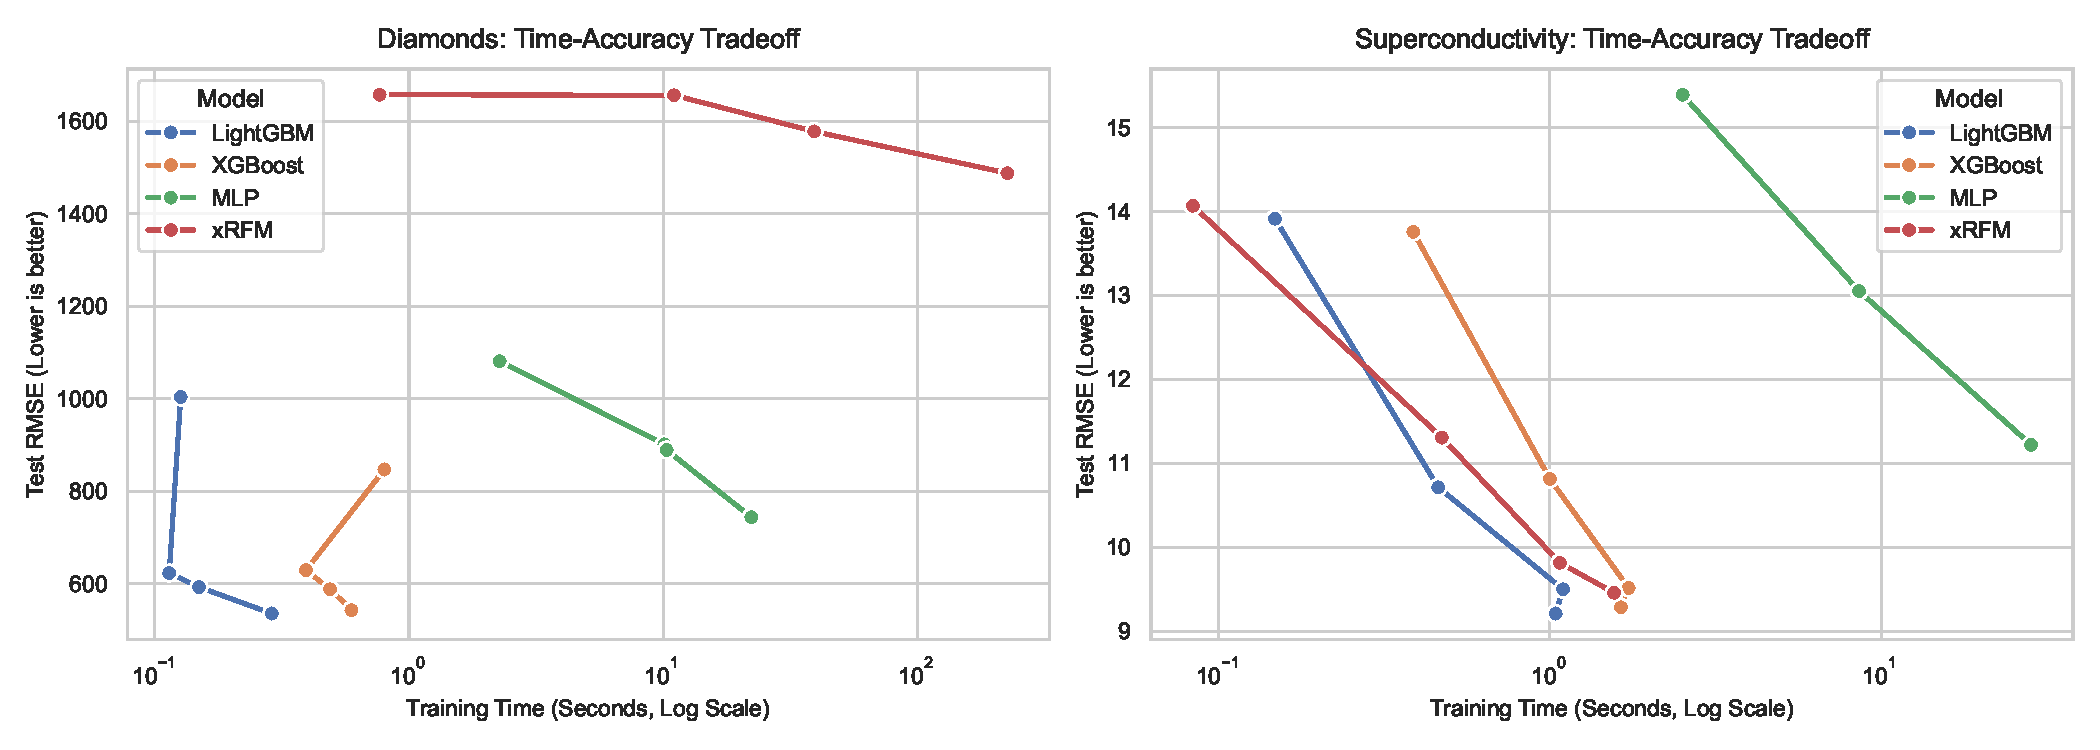
\includegraphics[width=\textwidth]{figures/time_accuracy_tradeoff.pdf}
  \caption{Time-Accuracy tradeoff comparison. The points for each model represent different training sizes ($n$). This visualization highlights the efficiency gap between AGOP reweighting and gradient boosting.}
  \label{fig:tradeoff}
\end{figure}

\subsection{Interpretability Comparison}

Figure~\ref{fig:feature-importance} visualises the top-five AGOP-ranked features extracted from the trained xRFM models for representative datasets.

\begin{figure}[htbp]
  \centering
  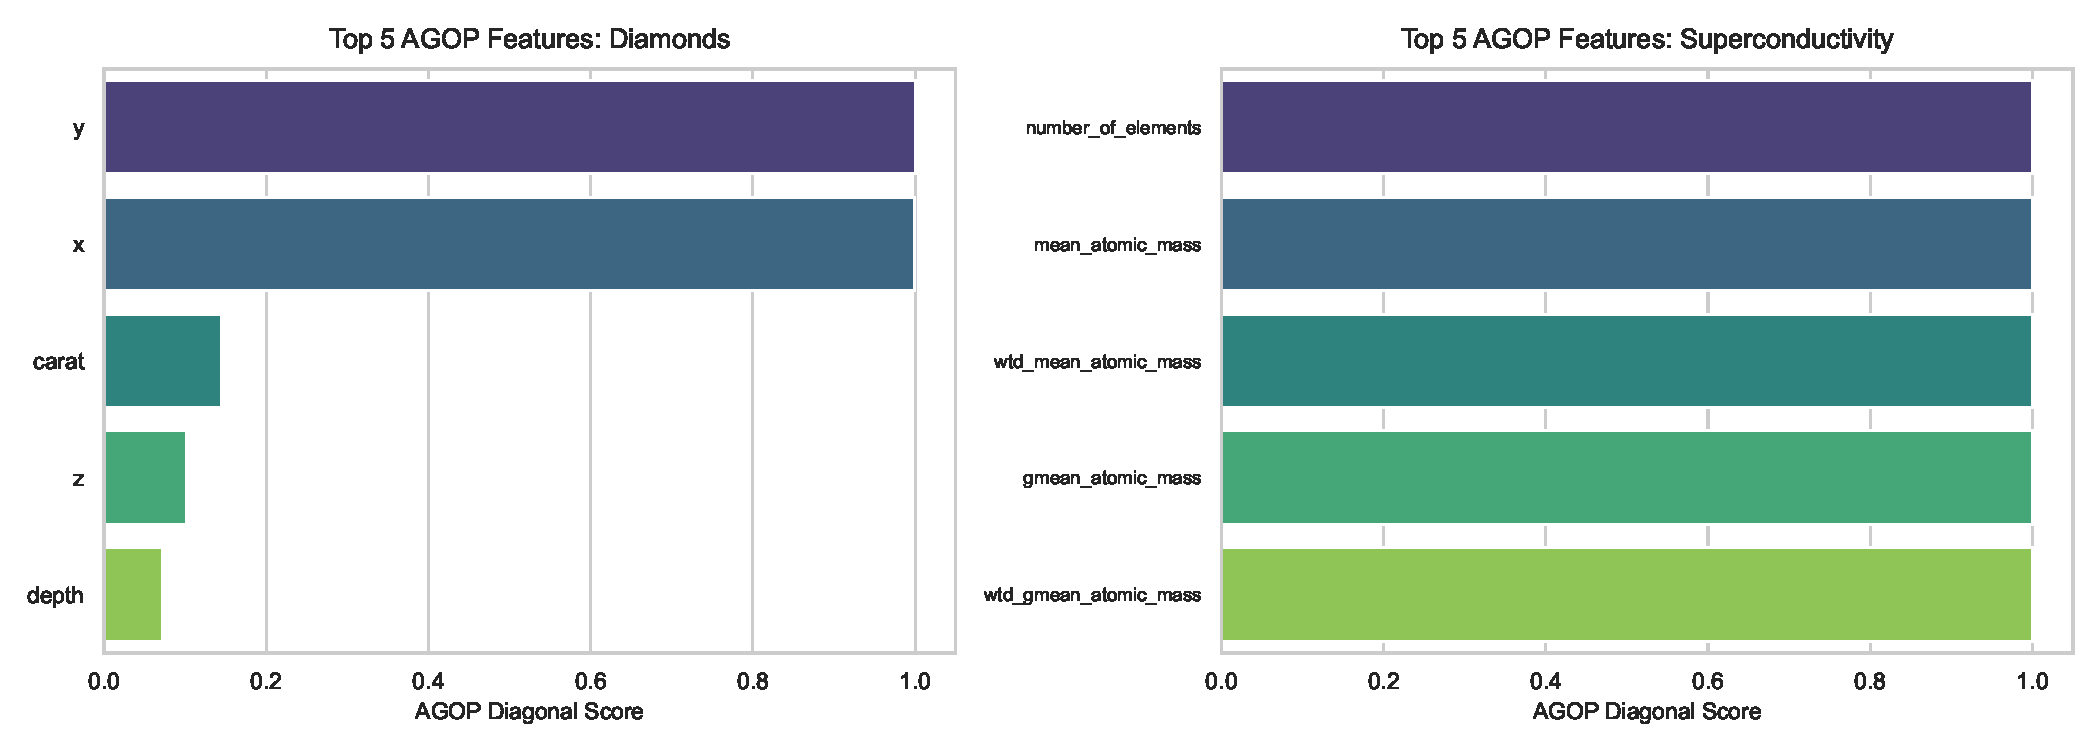
\includegraphics[width=\textwidth]{figures/feature_importance_bars.pdf}
  \caption{Top 5 feature importance rankings derived from the xRFM AGOP diagonal values for the Diamonds and Superconductivity datasets.}
  \label{fig:feature-importance}
\end{figure}

The AGOP rankings are broadly interpretable: physical size variables ($x, y, z$) for Diamonds and atomic mass variables for Superconductivity all align with domain knowledge[cite: 122]. Notably, the dominance of \texttt{y} and \texttt{x} in Diamonds reflects the learned function's high sensitivity to these continuous dimensions, despite the model's overall predictive lag behind GBDTs.

Table~\ref{tab:interpretability-methods} compares AGOP diagonal importance with PCA, mutual information, and permutation importance. These methods answer different questions.

\begin{table}[htbp]
  \centering
  \caption{Conceptual comparison of interpretability methods for tabular features.}
  \label{tab:interpretability-methods}
  \small
  \begin{tabular}{llll}
    \toprule
    Method & Supervised? & Model-specific? & Main interpretation \\
    \midrule
    AGOP diagonal          & Yes & Yes            & Sensitivity of xRFM to each feature \\
    PCA loadings           & No  & No             & Directions of maximum input variance \\
    Mutual information     & Yes & No             & Feature-target dependence \\
    Permutation importance & Yes & Model-agnostic & Performance drop after feature shuffle \\
    \bottomrule
  \end{tabular}
\end{table}

Notably, meaningful AGOP rankings do not imply strong predictive performance: on Diamonds, AGOP identifies sensible size-related features, yet xRFM's RMSE is nearly three times higher than LightGBM's[cite: 128]. This suggests that boosted trees capture axis-aligned thresholds more efficiently than AGOP reweighting, and that interpretability and accuracy can be decoupled[cite: 129].
